\documentclass[11pt]{report}

%-------------PACOTES-----------------%
\usepackage[latin1,utf8]{inputenc}
\usepackage[portuguese]{babel}
\usepackage[nottoc,notlot,notlof]{tocbibind}
\usepackage{graphicx}
\usepackage{float}
\usepackage{caption}
\usepackage{subcaption}
\usepackage{booktabs}
\usepackage{colortbl}
\usepackage{titlepic}
\usepackage{amsmath}
\usepackage{amssymb}
\usepackage[margin=1.0in]{geometry}
\usepackage{titlesec}
\titleformat{\chapter}[display]
{\normalfont\huge\bfseries}{\chaptertitlename\ \thechapter}{20pt}{\Huge}
\titlespacing*{\chapter}{0pt}{-50pt}{40pt}


%-------------------------------------%

\begin{document}

%-------------CAPA--------------------%
\titlepic{
\includegraphics[scale=0.5]{logoCiencias}}
\title{Força Electromotriz Induzida}
\author{João Olívia 52875\\
		Ernesto González 52857\\}
\date{Física Experimental II\\
	  Faculdade de Ciências - Universidade de Lisboa\\
	  Ano Letivo 2019/2020}

\maketitle
%-------------------------------------%
%-------------ÍNDICE------------------%
\tableofcontents
%-------------------------------------%
%-------------RESUMO------------------%
\chapter{Resumo}
Estudo da força eletromotriz induzida num circuito acoplado a uma calha em arrastamento. Análise da relação entre a força eletromotriz induzida no circuito pelo movimento da calha e os seguintes parâmetros: largura do circuito; raio de enrolamento do fio de arrastamento; número de ímanes. A calha inicialmente inserida no suporte onde se encontram os ímanes é movida com velocidade constante através de um motor com um suporte ao qual está conectada por um fio. O suporte é constituído por cilindros de diferentes raios o que permitiu a obtenção de diferentes velocidades de arrastamento da barra para a mesma velocidade angular do motor. Foram registados os diferentes parâmetros mencionados acima e feita a análise da relação entre a força eletromotriz induzida e estes. Os resultados da análise estão em concordância com os valores teóricos esperados uma vez que foi verificada a relação de  porporcionalidade direta entre a força eletromotriz e todas as três variáveis.
%-------------------------------------%
%-------------INTRODUÇÃO--------------%
\chapter{Introdução}
\textit{Para assegurar uma corrente eléctrica num circuito fechado é necessário despender energia} [4**]. Neste caso a energia referida vem do motor que possibilita o movimento da barra. A energia mecânica proveniente do motor manifesta-se na energia cinética da barra que, ao fazer variar a posição do circuito em relação aos ímans e portanto a área, induz a força eletromotriz no mesmo. Esta influência da variação da área e da velocidade da barra na indução da força eletromotriz é explicada pelas seguintes equações:

\begin{center}
    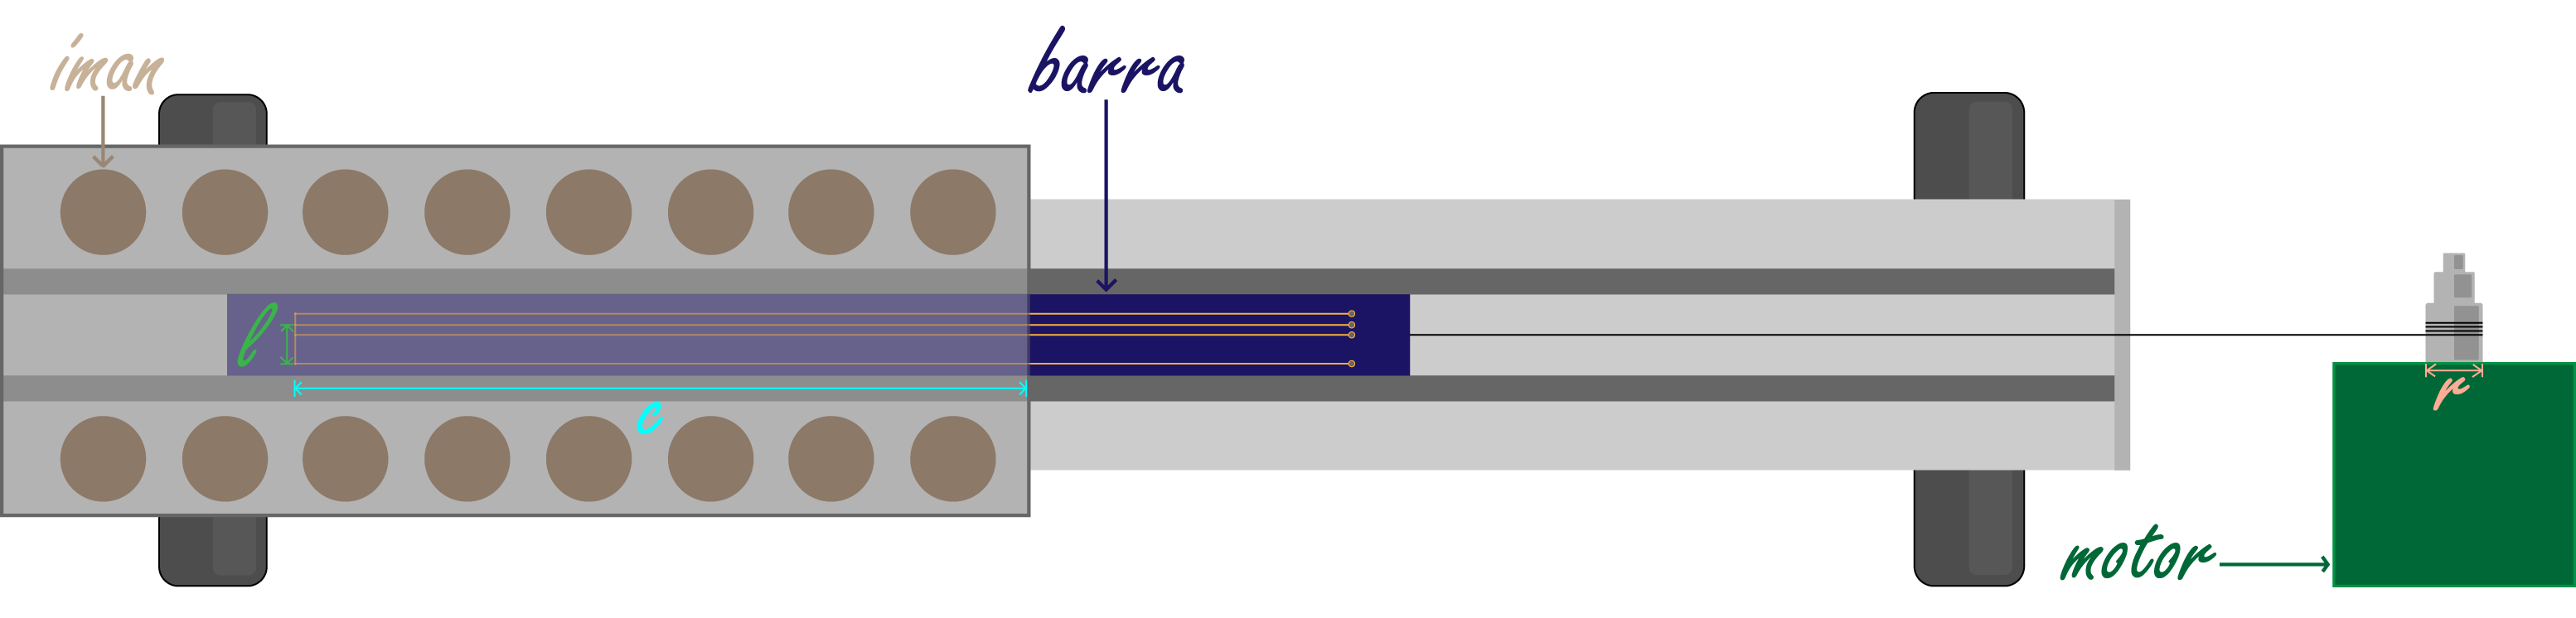
\includegraphics[width=0.8\textwidth]{FIGBARRA.png}
\captionof{figure}{Animação da montagem onde estão assinaladas as variáveis l$\ell$ e c, representando a largura do circuito e o comprimento da porção da barra dentro da estrutura, respetivamente.}
    \label{fig:mc-1}
\end{center}

\begin{equation} \epsilon = \oint \overrightarrow{E}.\overrightarrow{d\ell} = \oint \frac{\overrightarrow{F}}{q}.\overrightarrow{d\ell} = \oint(\overrightarrow{v} \times \overrightarrow{B}).\overrightarrow{d\ell}\end{equation}
Uma vez que o circuito está em movimento em relação aos ímans então o integral de linha em (2.1) pode ser escrito da seguinte forma:\\
\begin{equation}
	\oint(\overrightarrow{v} \times \overrightarrow{B}).\overrightarrow{d\ell} = \int_{-\ell}(\overrightarrow{v} \times \overrightarrow{B}).\overrightarrow{d\ell} + \int_{\ell} (\overrightarrow{v} \times \overrightarrow{B}).\overrightarrow{d\ell} + \int_{c} (\overrightarrow{v} \times \overrightarrow{B}).\overrightarrow{d\ell} + \int_{-c}(\overrightarrow{v} \times \overrightarrow{B}).\overrightarrow{d\ell}
\end{equation}
Como a velocidade é nula na barra ($\ell$) tem-se que:
\begin{equation}
	\int_{\ell} (\overrightarrow{v} \times \overrightarrow{B}).\overrightarrow{d\ell} = 0\end{equation}
Pelo que de (2.2) vem:
\begin{equation}\oint(\overrightarrow{v} \times \overrightarrow{B}).\overrightarrow{d\ell} = \int_{-\ell}(\overrightarrow{v} \times \overrightarrow{B}).\overrightarrow{d\ell} +  \int_{c} (\overrightarrow{v} \times \overrightarrow{B}).\overrightarrow{d\ell} + \int_{-c} (\overrightarrow{v} \times \overrightarrow{B}).\overrightarrow{d\ell}
\end{equation}
Uma vez que os dois últimos integrais de (2.4) são simétricos:
\begin{equation}
	\epsilon = \oint(\overrightarrow{v} \times \overrightarrow{B}).\overrightarrow{d\ell} = \int_{-\ell}(\overrightarrow{v} \times \overrightarrow{B}).\overrightarrow{d\ell} = vB\ell=\frac{\partial (Bc\ell)}{\partial t}= \frac{\partial \Phi}{\partial t}
\end{equation}

Tendo em conta que $v=\omega r$, de (2.5) vem
\begin{equation}
	\epsilon = \omega rB\ell
\end{equation}

%-------------------------------------%
%---------MÉTODO E EQUIPAMENTO--------%
\chapter{Procedimento e Equipamento}
\textbf{Material utilizado:}
\begin{itemize}
\item Aparelho de indução com 3 espiras móveis
\item Motor e unidade de comando
\item Conjunto de 16 ímanes permanentes
\item Amplificador de tensão
\item Galvanómetro, régua e cronómetro
\end{itemize}
\textbf{Procedimento:}
\begin{itemize}
\item Começou por se acertar a velocidade de arrastamento da barra em aproximadamente 1 $cm.s^{-1}$ (O objetivo deste acerto é evitar uma velocidade linear muito elevada com o aumento do raio do suporte o que poderia afetar a medição do valor da força eletromotriz.) Para a realização do dito acerto foi usado o cronómetro com a finalidade de medir o tempo que a barra demora a percorrer o comprimento da calha., uma vez que a velocidade desejada é 1 $cm.s^{-1}$ então o valor do tempo desejado em segundos é igual ao comprimento da calha em centímetros.
\item Fixou-se o número de ímanes no suporte e fizeram-se as medições da força eletromotriz com o auxílio do galvanómetro e do amplificador de tensão fazendo variar a velocidade de arrastamento e a largura do circuito. Repetiu-se este processo para 4, 6, 8, 10, 12 e 16 ímanes.


\end{itemize}
%-------------------------------------%
%-------------RESULTADOS--------------%
\chapter{Resultados}
Durante toda a experiência usou-se $\omega=1112\pm0.05\;rad\,s^{-1}.$\\
De (2.6) vem
\begin{equation}
	\epsilon = \omega rB\ell
\end{equation}
Portanto, se fixarmos a velocidade de arrastamento, ou seja, o raio de enrolamento do fio tem-se que:
\begin{equation}
	\epsilon = \epsilon(\ell)
\end{equation}
Uma vez que $\epsilon$(f.e.m.i) é uma função da largura do circuito então o declive da reta (m) é dado por:
\begin{equation}
	m = \frac{\epsilon}{\ell}
\end{equation}
Pelo que de (4.1) vem:
\begin{equation}
	\frac{\epsilon}{\ell} = m = \omega rB
\end{equation}
Resolvendo para B:
\begin{equation}
	B(r) = \frac{m}{\omega r}
\end{equation}

Ao analisar os gráficos e as respetivas tabelas podemos facilmente constatar que a razão entre os declives das três retas é igual à razão entre os raios de enrolamento correspondentes à respetiva função o que confirma a validade dos resultados experimentais obtidos. Os declives positivos em todas as retas de todos os gráficos são a confirmação experimental de que a força eletromotriz induzida é diretamente proporcional à largura do circuito.

\begin{figure}[H]
\centering
\begin{subfigure}{.5\textwidth}
  \centering
  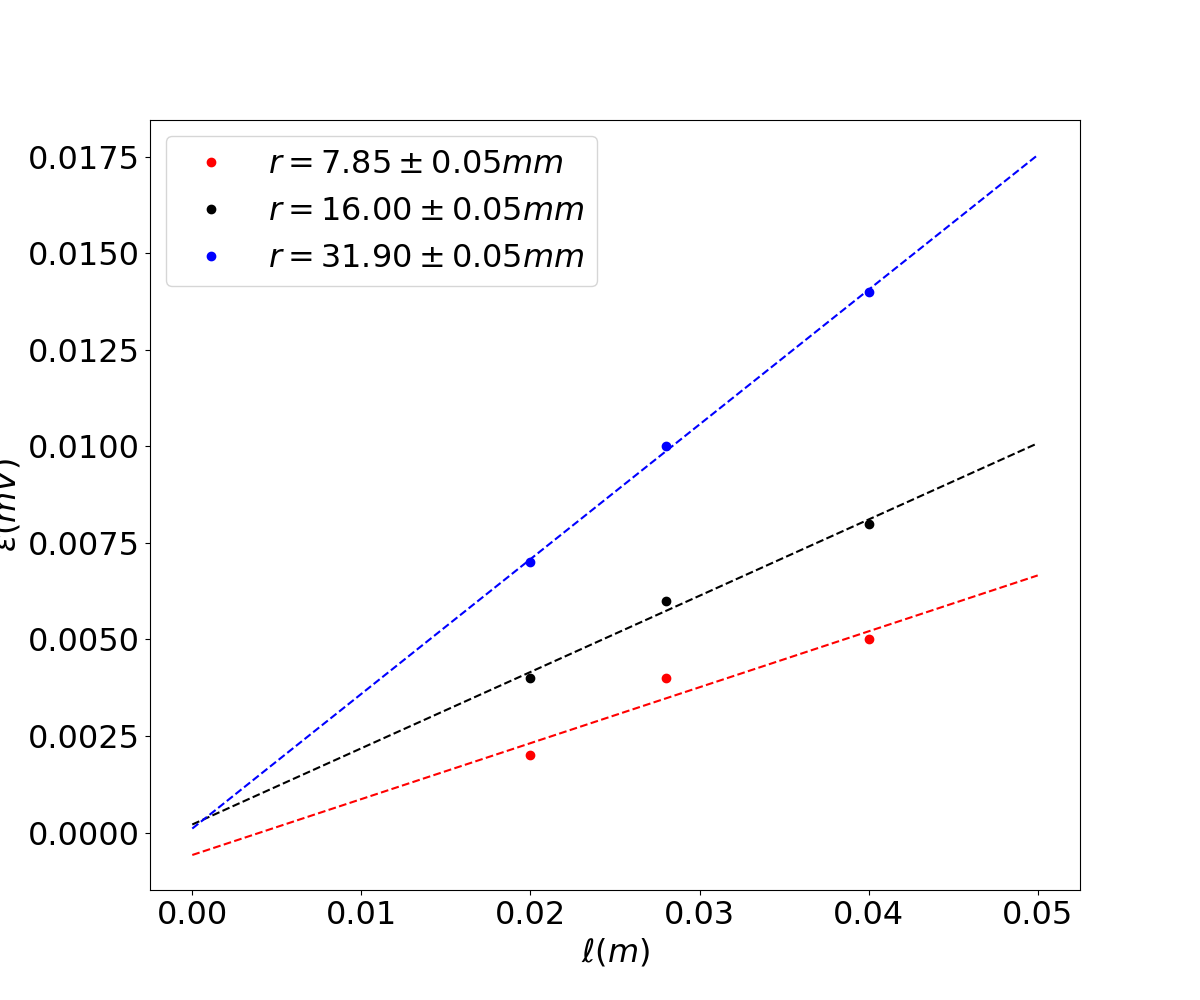
\includegraphics[width=1\linewidth]{i4lfem.png}
  \caption{4 ímanes}
  \label{fig:sub1}
\end{subfigure}%
\begin{subfigure}{.5\textwidth}
  \centering
  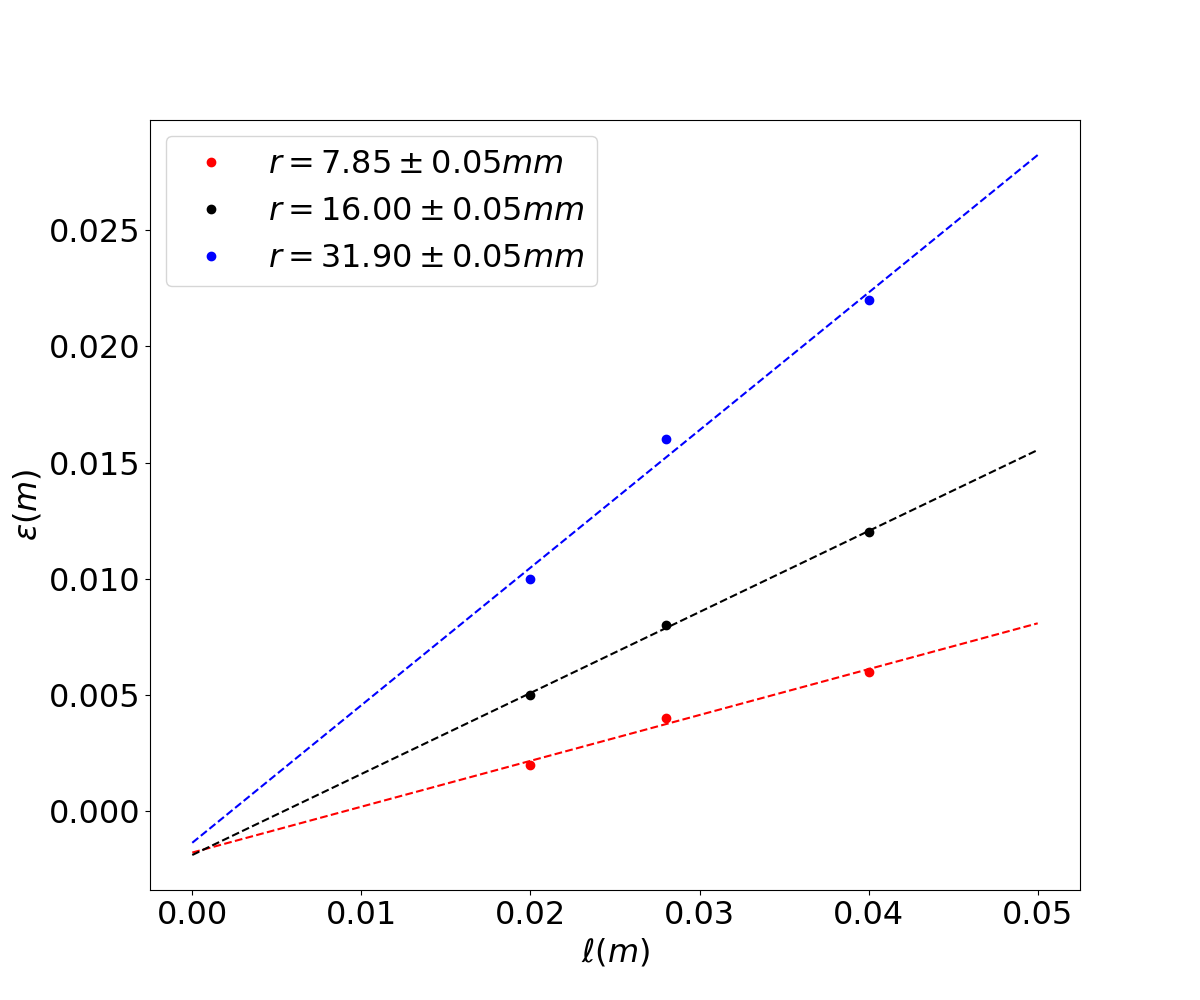
\includegraphics[width=1\linewidth]{i6lfem.png}
  \caption{6 ímanes}
  \label{fig:sub2}
\end{subfigure}
\begin{subfigure}{.5\textwidth}
  \centering
  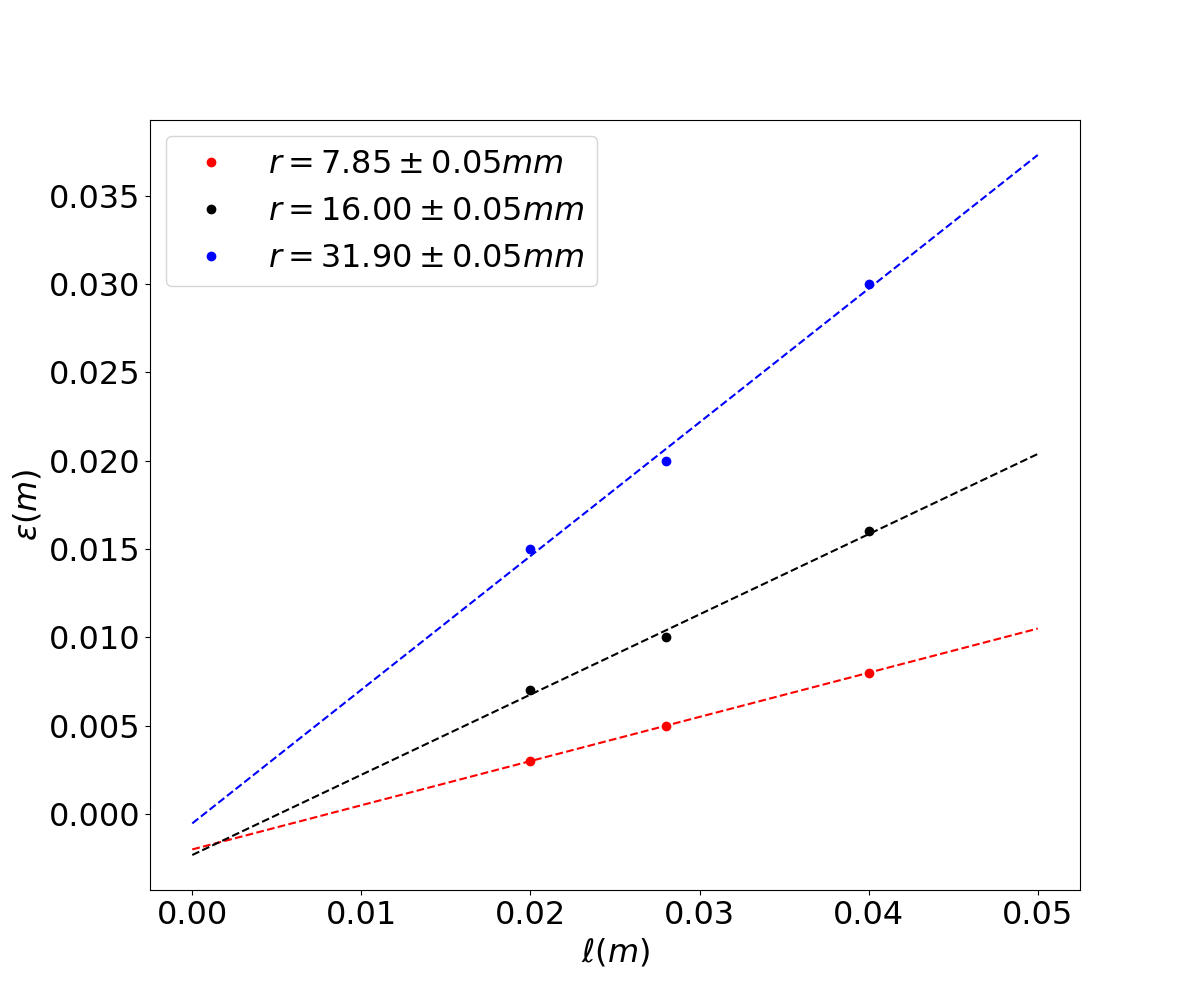
\includegraphics[width=1\linewidth]{i8lfem.png}
  \caption{8 ímanes}
  \label{fig:sub2}
\end{subfigure}%
\begin{subfigure}{.5\textwidth}
  \centering
  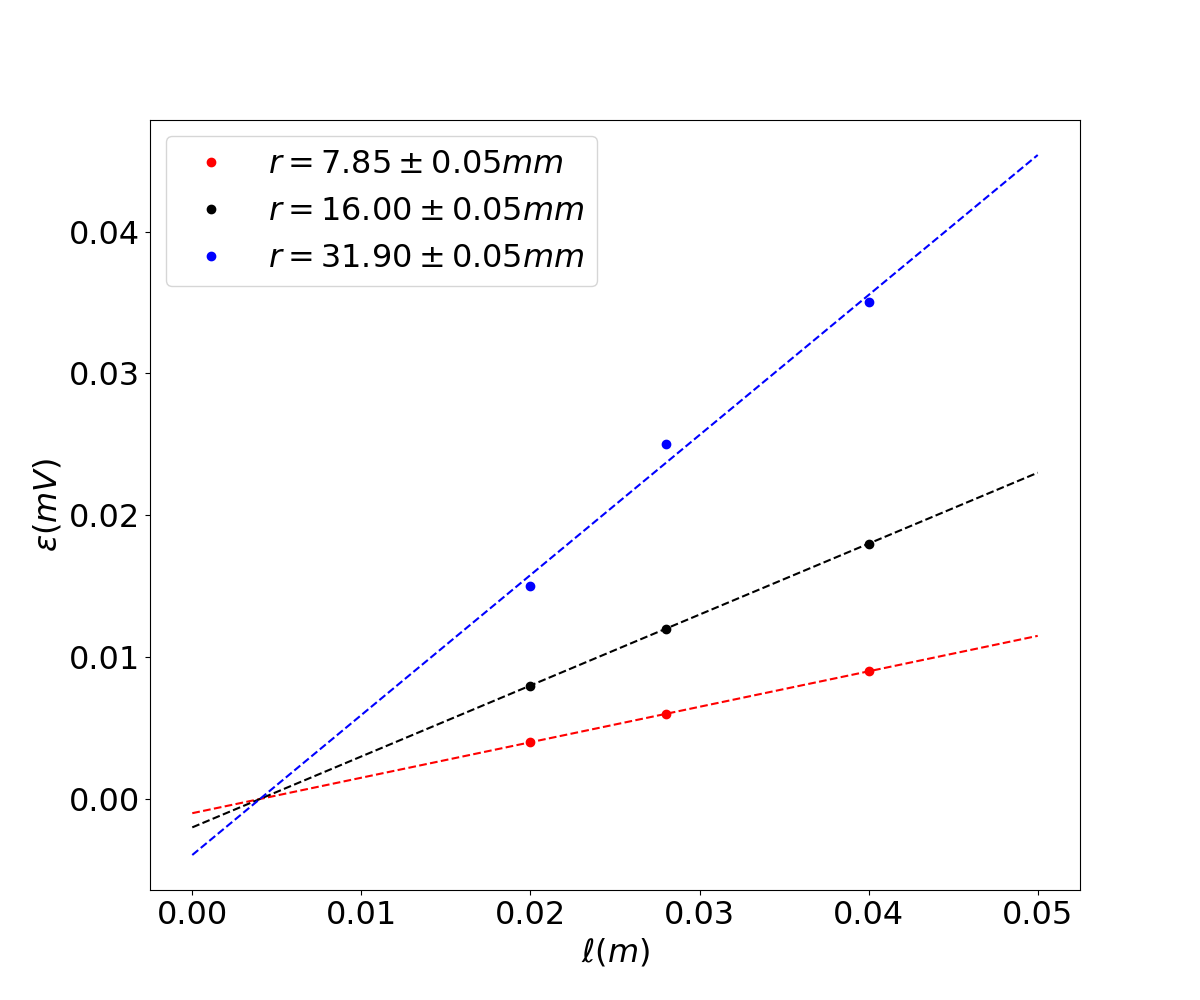
\includegraphics[width=1\linewidth]{i10lfem.png}
  \caption{10 ímanes}
  \label{fig:sub2}
\end{subfigure}
\begin{subfigure}{.5\textwidth}
  \centering
  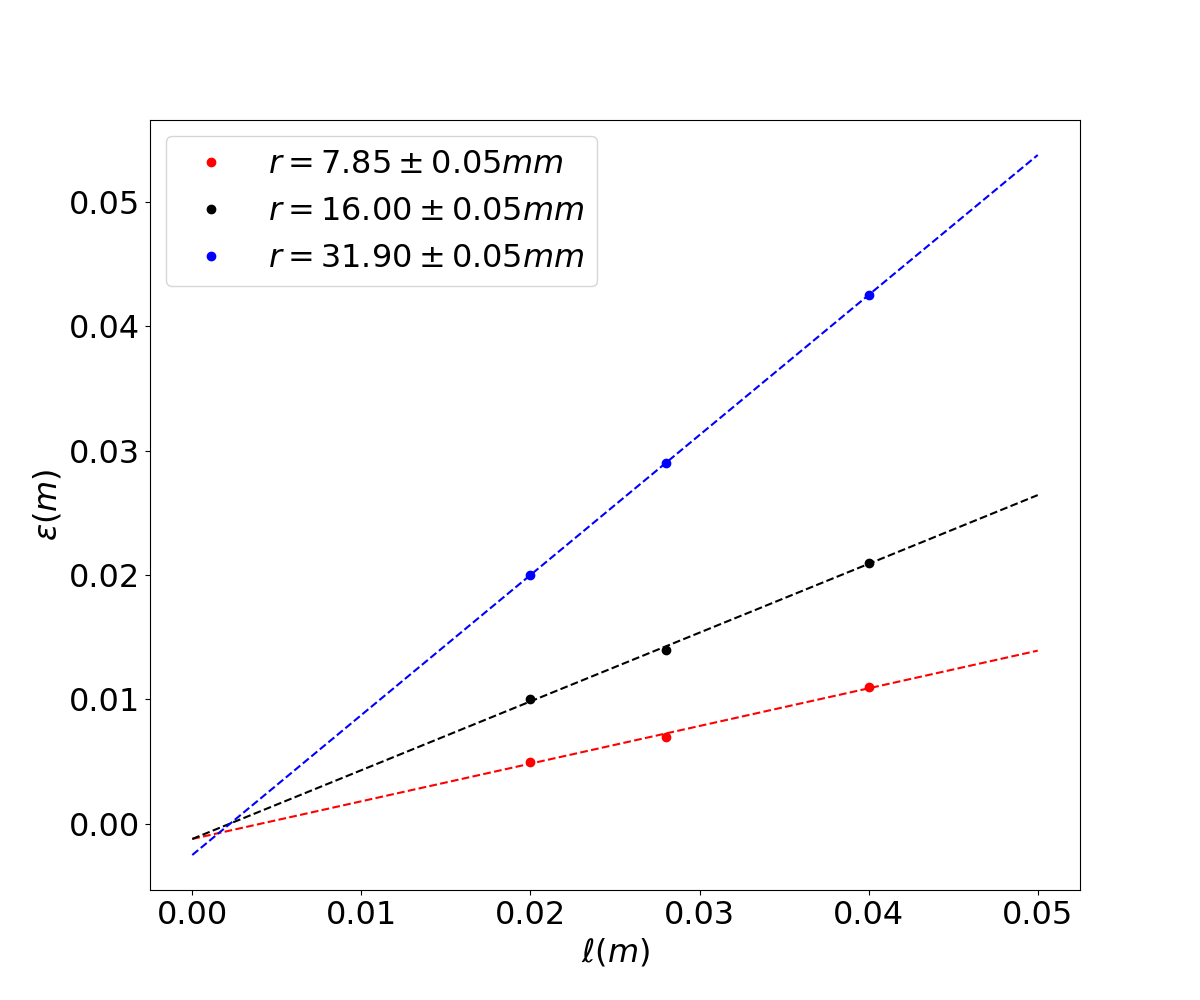
\includegraphics[width=1\linewidth]{i12lfem.png}
  \caption{12 ímanes}
  \label{fig:sub2}
\end{subfigure}%
\begin{subfigure}{.5\textwidth}
  \centering
  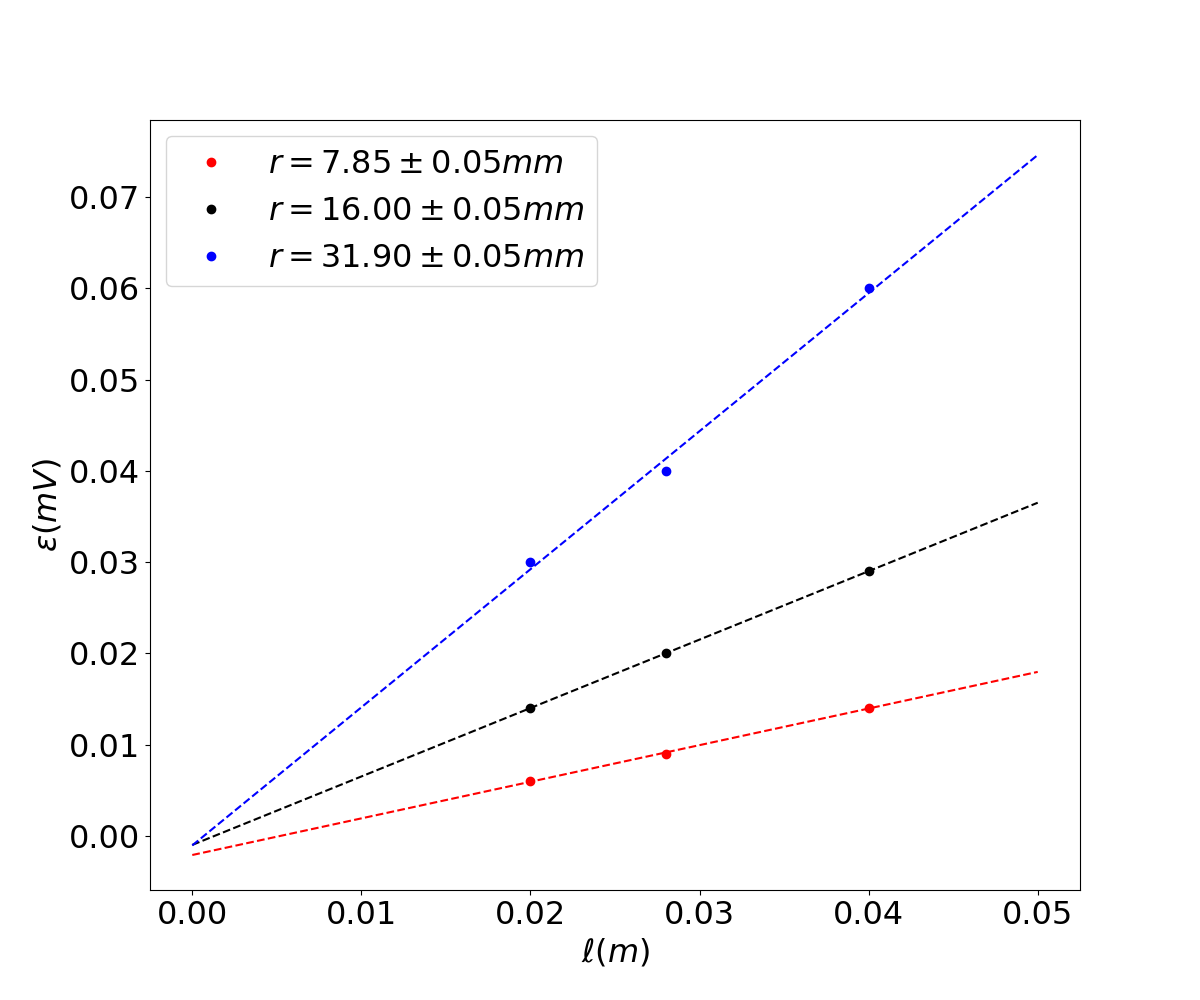
\includegraphics[width=1\linewidth]{i16lfem.png}
  \caption{16 ímanes}
  \label{fig:sub2}
\end{subfigure}
\label{fig:test}
\caption{Nas 6 figuras encontra-se representado $\epsilon(\ell)$ para $r=7.85\pm0.05mm$, $r=16.00\pm0.05mm$ e $r=31.90\pm0.05mm$ para as 6 configurações de números de ímanes: 4, 6 ,8 ,10, 12, 16.}
\end{figure}

\begin{table}[!htb]
	\caption{Tabelas com os declives das retas da Figura 4.1. Uma tabela para cada configuração de número de ímanes. Cada tabela indica o declive da reta a que corresponde o respetivo raio e a intensidade total do campo magnético, estimada a partir de $\frac{m}{\omega r}$ em que $m$ é o declive da reta e $r$ o raio.}
	\vspace{\abovedisplayskip}
		\begin{minipage}{.5\linewidth}
			\centering
			\caption{4 ímanes, $\overline{B} = 3.47532334 mT$}
				\begin{tabular}{lllll}
	\hline
	Declive        & raio(r)(mm)     & B(mT)           \\ \hline
	0.14473684 & $7.85\pm 0.05$   & 18.43751425  \\
	0.19736842 & $16.00\pm 0.05$   & 12.33552632\\
	0.34868421 & $31.90\pm 0.05$    & 13.90129337   \\ \hline
				\end{tabular}
		\end{minipage}%
		\vspace{\belowdisplayskip}
		\vspace{\abovedisplayskip}
		\begin{minipage}{.5\linewidth}
			\centering
			\caption{6 ímanes, $\overline{B} = 3.63869615 mT$}
				\begin{tabular}{lllll}
	\hline
	Declive        & raio(r)(mm)     & B(mT)           \\ \hline
	0.19736842& $7.85\pm 0.05$   & 25.14247402  \\
	0.34868421& $16.00\pm 0.05$   & 21.79276316\\
	0.59210526& $31.90\pm 0.05$    & 18.56129352   \\ \hline
				\end{tabular}
		\end{minipage}
		\vspace{\belowdisplayskip}
		\vspace{\abovedisplayskip}
		\begin{minipage}{.5\linewidth}
			\centering
			\caption{8 ímanes, $\overline{B} = 3.49733553 mT$}
				\begin{tabular}{lllll}
	\hline
	Declive        & raio(r)(mm)     & B(mT)           \\ \hline
	0.25000000 & $7.85\pm 0.05$   & 31.84713376  \\
	0.45394737& $16.00\pm 0.05$   & 28.37171053\\
	0.75657895& $31.90\pm 0.05$   & 23.71720838   \\ \hline
				\end{tabular}
		\end{minipage}%
		\vspace{\belowdisplayskip}
		\vspace{\abovedisplayskip}
		\begin{minipage}{.5\linewidth}
			\centering
				\caption{10 ímanes, $\overline{B} = 3.13442077 mT$}
				\begin{tabular}{lllll}
	\hline
	Declive        & raio(r)(mm)            & B(mT)           \\ \hline
	0.25000000 & $7.85\pm 0.05$                 & 31.84713376  \\
	0.50000000 & $16.00\pm 0.05$                & 31.2500000\\
	0.45502905 & $31.90\pm 0.05$  & 30.93548919   \\ \hline
				\end{tabular}
		\end{minipage}
		\vspace{\belowdisplayskip}
		\vspace{\abovedisplayskip}
		\begin{minipage}{.5\linewidth}
			\centering
			\caption{12 ímanes, $\overline{B} = 3.0099368 mT$}
				\begin{tabular}{lllll}
	\hline
	Declive        & raio(r)(mm)     & B(mT)          \\ \hline
	0.30263158 & $7.85\pm 0.05$  &38.5517935  \\
	0.55263158& $216.00\pm 0.05$      &34.53947368 \\
	1.12500000& $31.90\pm 0.05$    &35.26645768   \\ \hline
				\end{tabular}
		\end{minipage}%
		\vspace{\belowdisplayskip}
		\vspace{\abovedisplayskip}
		\begin{minipage}{.5\linewidth}
			\centering
			\caption{16 ímanes, $\overline{B} = 3.02984265 mT$}
				\begin{tabular}{lllll}
	\hline
	Declive        & raio(r)(mm)            & B(mT)           \\ \hline
	0.40131579 &$7.85\pm 0.05$      & 51.12303051  \\
	0.75000000 &$16.00\pm 0.05$   & 46.8750000\\
	1.51315789 &$31.90\pm 0.05$     & 47.43441676   \\ \hline
				\end{tabular}
		\end{minipage}
		\vspace{\belowdisplayskip}
\end{table}

À semelhança do que foi verificado para a situação anterior, através dos gráficos acima podemos verificar a relação de proporcionalidade direta entre a força eletromotriz induzida e o raio de enrolamento do fio.

Através dos valores apresentados na tabela 4.1 e da equação (4.5) foram calculados os campos magnéticos médios de cada íman para cada número de ímans, tendo os valores sido apresentados nas respetivas legendas.



Fixando agora a largura do circuito temos que a força eletromotriz induzida passa a ser uma função do raio de enrolamento do fio:
\begin{equation}
	\epsilon = \epsilon (r)
\end{equation}
Com isto e seguindo um raciocínio análogo àquele feito na situação anterior obtemos uma expressão para o valor do campo (B):

\begin{equation}
	B(\ell) = \frac{m}{\omega \ell}
\end{equation}



\begin{figure}[H]
	\centering
	\begin{subfigure}{.5\textwidth}
	  \centering
	  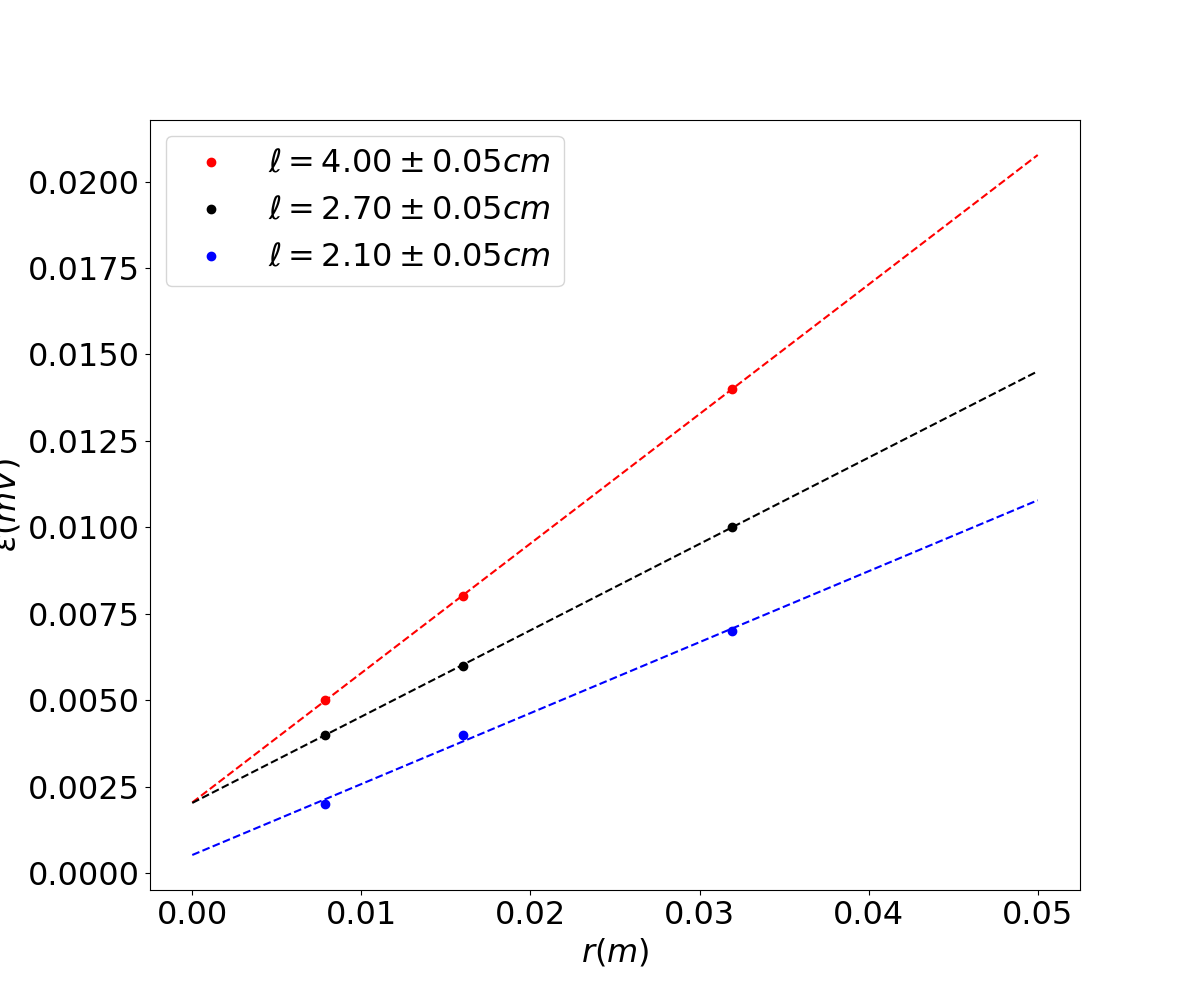
\includegraphics[width=1\linewidth]{i4rfem.png}
	  \caption{4 ímanes}
	  \label{fig:sub1}
	\end{subfigure}%
	\begin{subfigure}{.5\textwidth}
	  \centering
	  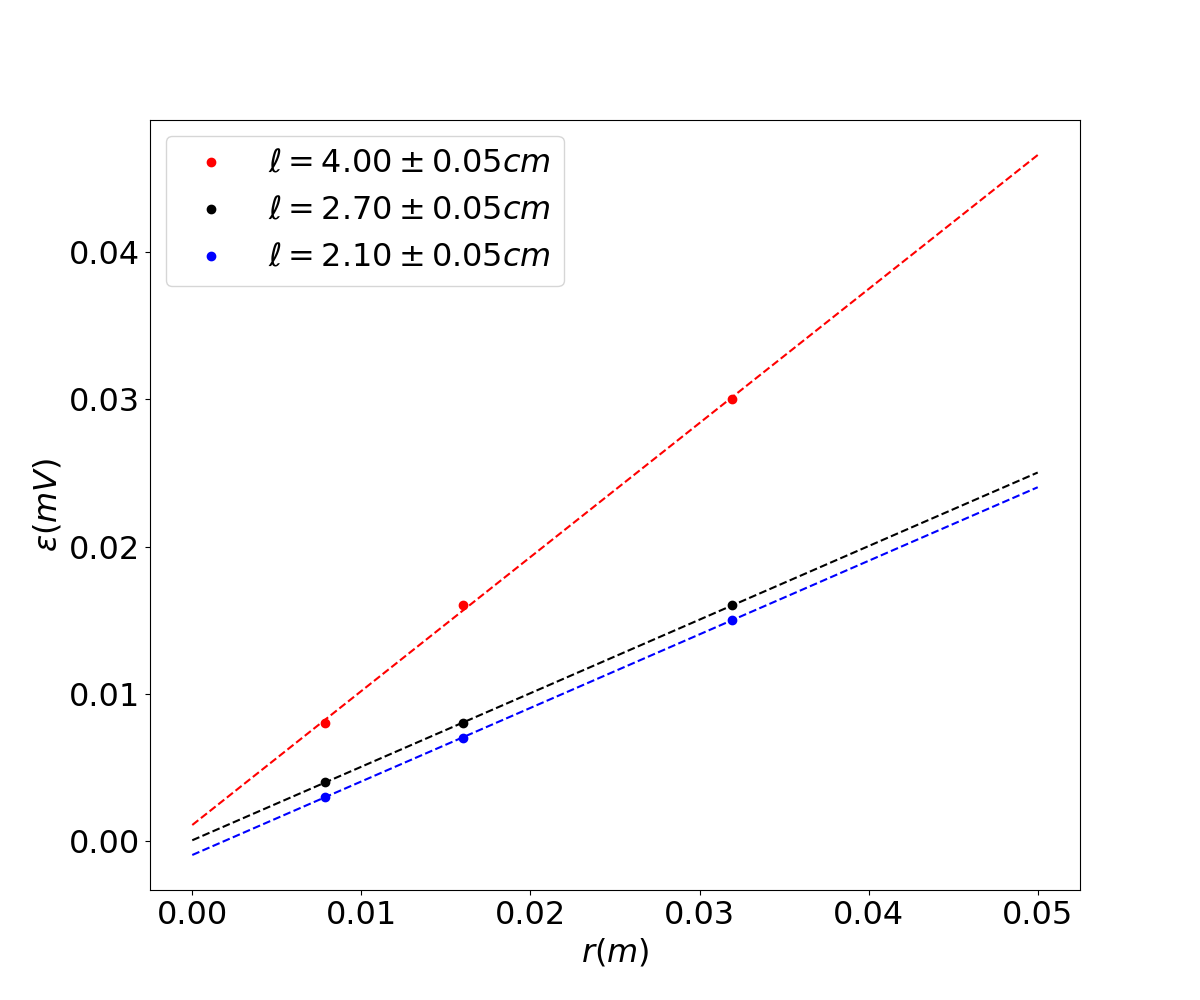
\includegraphics[width=1\linewidth]{i6rfem.png}
	  \caption{6 ímanes}
	  \label{fig:sub2}
	\end{subfigure}
	\begin{subfigure}{.5\textwidth}
	  \centering
	  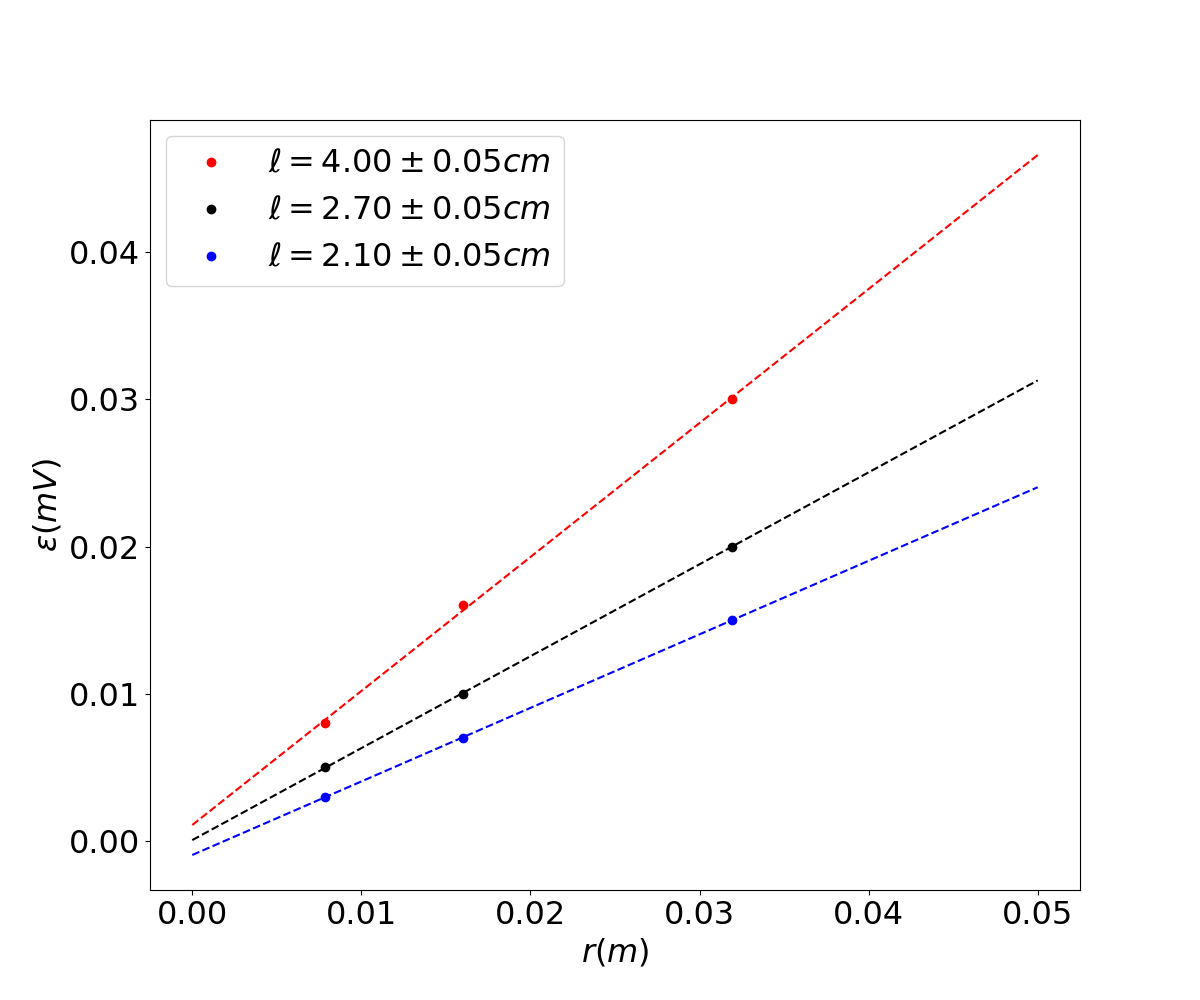
\includegraphics[width=1\linewidth]{i8rfem.png}
	  \caption{8 ímanes}
	  \label{fig:sub2}
	\end{subfigure}%
	\begin{subfigure}{.5\textwidth}
	  \centering
	  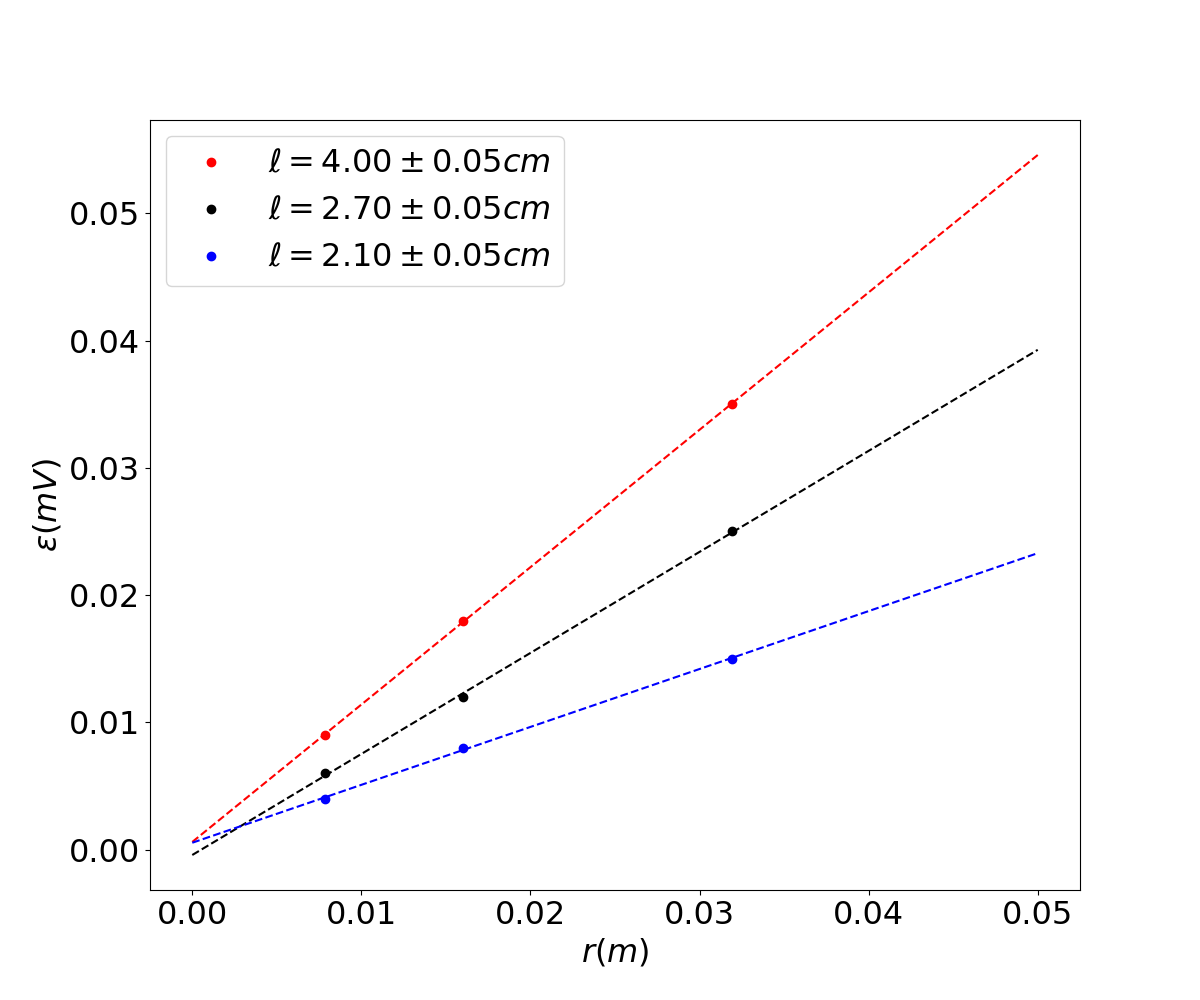
\includegraphics[width=1\linewidth]{i10rfem.png}
	  \caption{10 ímanes}
	  \label{fig:sub2}
	\end{subfigure}
	\begin{subfigure}{.5\textwidth}
	  \centering
	  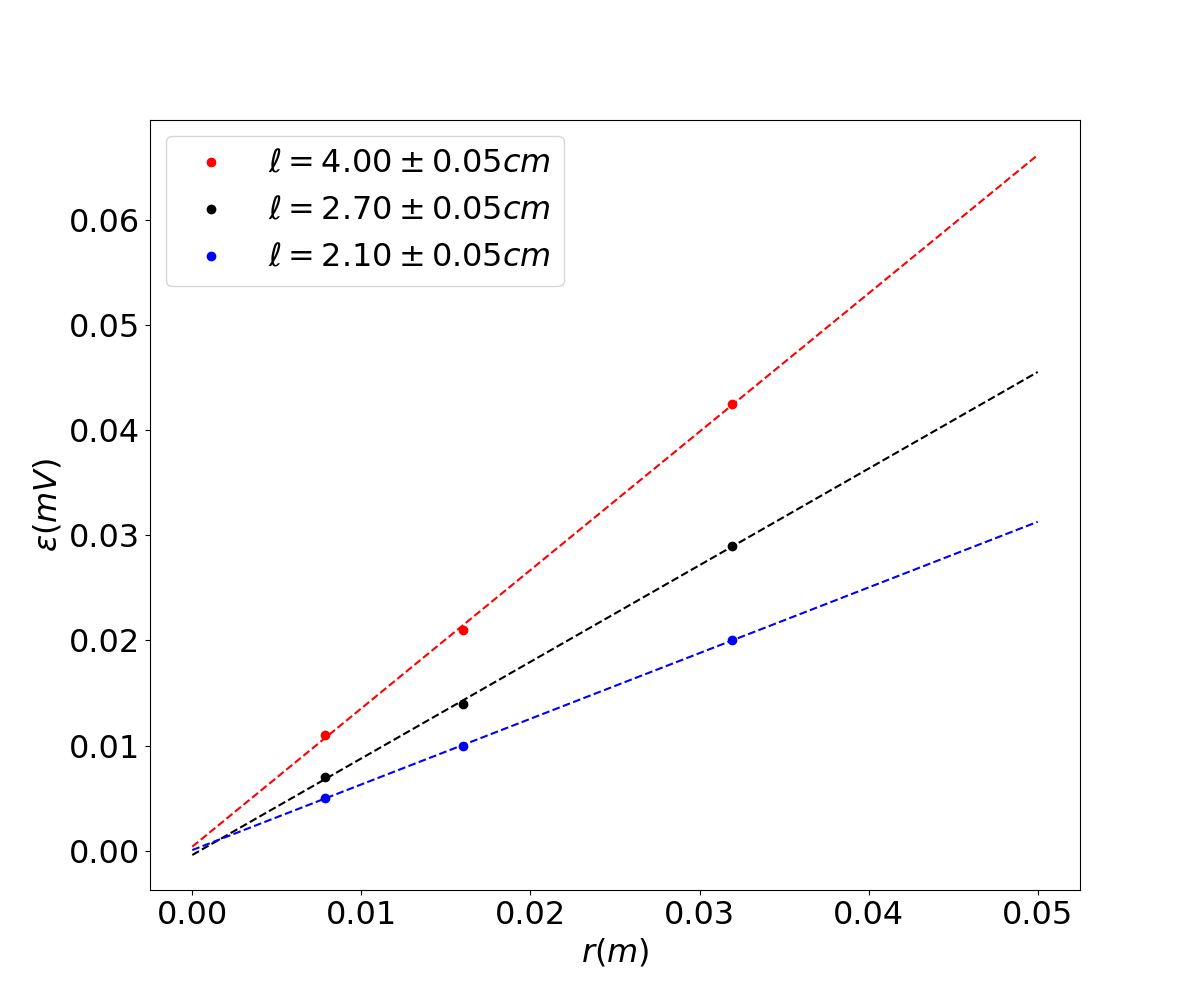
\includegraphics[width=1\linewidth]{i12rfem.png}
	  \caption{12 ímanes}
	  \label{fig:sub2}
	\end{subfigure}%
	\begin{subfigure}{.5\textwidth}
	  \centering
	  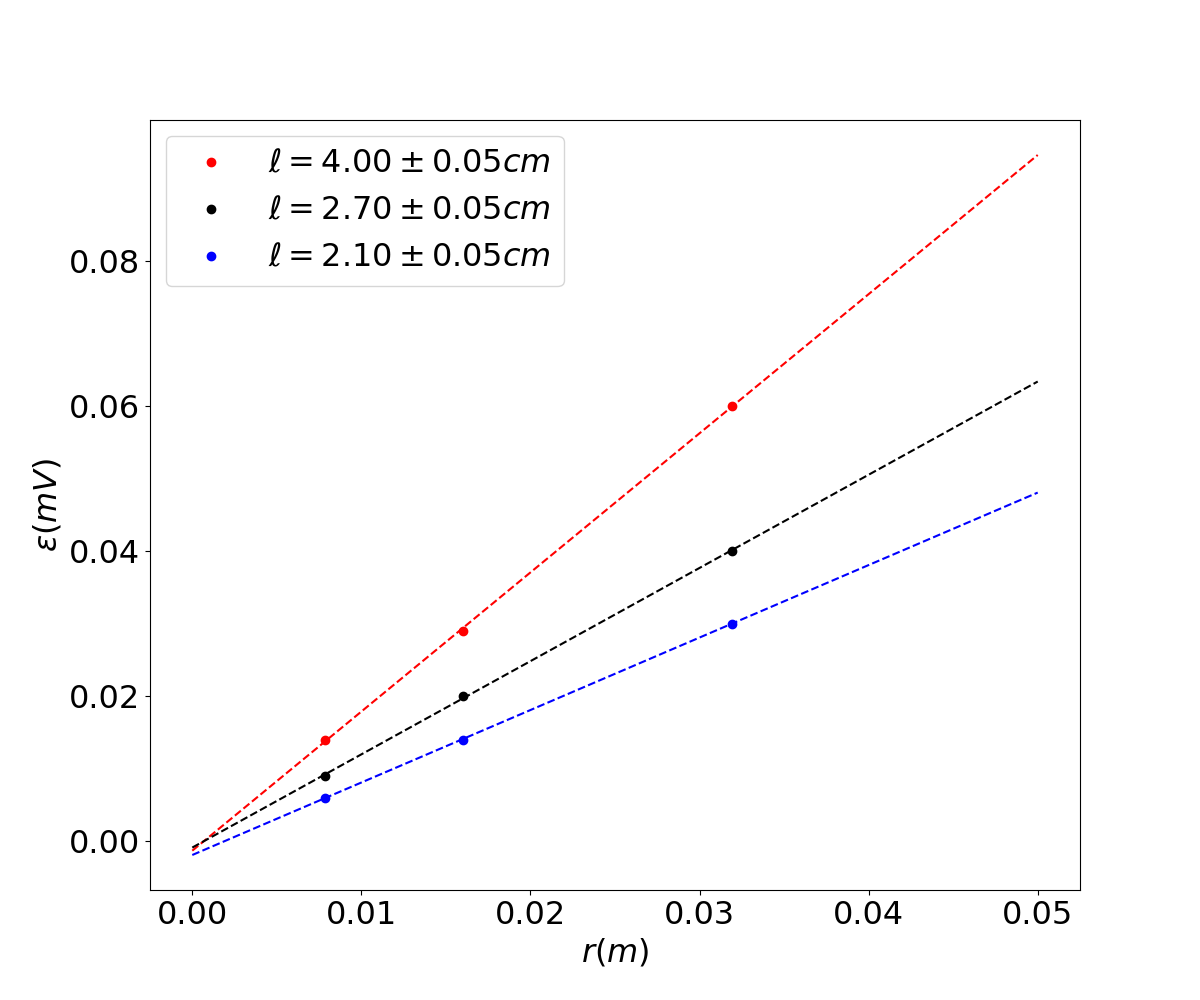
\includegraphics[width=1\linewidth]{i16rfem.png}
	  \caption{16 ímanes}
	  \label{fig:sub2}
	\end{subfigure}
	\label{fig:test}
	\caption{Nas 6 figuras encontra-se representado $\epsilon(\ell)$ para $\ell=2.1\pm0.05cm$, $r=2.70\pm0.05cm$ e $r=4.00\pm0.05cm$ para as 6 configurações de números de ímanes: 4, 6 ,8 ,10, 12, 16.}
	\end{figure}

	\begin{table}[!htb]
			\caption{Tabelas com os declives das retas da Figura 4.1. Uma tabela para cada configuração de número de ímanes. Cada tabela indica o declive da reta a que corresponde a respetiva largura e a intensidade total do campo magnético, estimada a partir de $\frac{m}{\omega \ell}$ em que $m$ é o declive da reta e $\ell$ a largura.}
		\vspace{\abovedisplayskip}
	    \begin{minipage}{.5\linewidth}
	      \centering
				\caption{4 ímanes, $\overline{B} = 2.36594061 mT$ }
	        \begin{tabular}{lllll}
		\hline
		Declive        & largura($\ell$)(cm)     & B(mT)           \\ \hline
		0.37465117 &$4.00\pm 0.05$   & 9.3662791  \\
		0.24976744&$2.70\pm 0.05$   & 9.25064609\\
		0.20526160&$2.10\pm 0.05$    & 9.7743621   \\ \hline
	        \end{tabular}
	    \end{minipage}%
			\vspace{\belowdisplayskip}
			\vspace{\abovedisplayskip}
	    \begin{minipage}{.5\linewidth}
	      \centering
				\caption{6 ímanes, $\overline{B} = 3.47532334 mT$}
	        \begin{tabular}{lllll}
		\hline
		Declive        & largura($\ell$)(cm)     & B(mT)           \\ \hline
		0.91005810 &$4.00\pm 0.05$   &22.75145243  \\
		0.49953489&$2.70\pm 0.05$  &18.50129218 \\
		0.49953489&$2.10\pm 0.05$  &23.78737566   \\ \hline
	        \end{tabular}
	    \end{minipage}
			\vspace{\belowdisplayskip}
			\vspace{\abovedisplayskip}
	    \begin{minipage}{.5\linewidth}
	      \centering
				\caption{8 ímanes, $\overline{B} = 2.9027268 mT$}
	        \begin{tabular}{lllll}
		\hline
		Declive        & largura($\ell$)(cm)     & B(mT)           \\ \hline
		0.91005810&$4.00\pm 0.05$   &22.75145243  \\
		0.62441861&$2.70\pm 0.05$  &23.12661523 \\
		0.34868421&$2.10\pm 0.05$  &23.78737566   \\ \hline
	        \end{tabular}
	    \end{minipage}%
			\vspace{\belowdisplayskip}
			\vspace{\abovedisplayskip}
	    \begin{minipage}{.5\linewidth}
	      \centering
				\caption{10 ímanes, $\overline{B} = 2.60181814 mT$}
	        \begin{tabular}{lllll}
		\hline
		Declive        & largura($\ell$)(cm)     & B(mT)           \\ \hline
		1.07944766 &$4.00\pm 0.05$  &26.98619149  \\
		0.79380817&$2.70\pm 0.05$   &29.40030273 \\
		0.45502905&$2.10\pm 0.05$  &21.66804993   \\ \hline
	        \end{tabular}
	    \end{minipage}
			\vspace{\belowdisplayskip}
			 \vspace{\abovedisplayskip}
	    \begin{minipage}{.5\linewidth}
	      \centering
				\caption{12 ímanes, $\overline{B} = 2.68471514 mT$}
	        \begin{tabular}{lllll}
		\hline
		Declive        & largura($\ell$)(cm)     & B(mT)          \\ \hline
		1.31559598 &$4.00\pm 0.05$  &32.88989957  \\
		0.91869190&$2.70\pm 0.05$     &34.02562578 \\
		0.62441861&$2.10\pm 0.05$   &32.21658164   \\ \hline
	        \end{tabular}
	    \end{minipage}%
			\vspace{\belowdisplayskip}
			\vspace{\abovedisplayskip}
	    \begin{minipage}{.5\linewidth}
	      \centering
				\caption{16 ímanes, $\overline{B} = 2.98126287 mT$}
	        \begin{tabular}{lllll}
		\hline
		Declive        & largura($\ell$)(cm)     & B(mT)           \\ \hline
		1.91776167 &$4.00\pm 0.05$   &47.94404184  \\
		1.28470926&$2.70\pm 0.05$   &47.58182458 \\
		0.99906978&$2.10\pm 0.05$   &47.57475132   \\ \hline
	        \end{tabular}
	    \end{minipage}
	\end{table}

	Ao analisar os gráficos conseguimos facilmente verificar a relação de proporcionalidade direta entre a força eletromotriz e a largura do circuito, uma vez que a função que descreve a relação entre as duas últimas variáveis mencionadas é positivo para qualquer configuração de ímanes.

	Através dos valores apresentados na tabela 4.8 e da equação (4.7) foram calculados os campos magnéticos médios de cada íman para cada número de ímans, tendo os valores sido apresentados nas respetivas legendas.


\begin{figure}[H]
	\center
	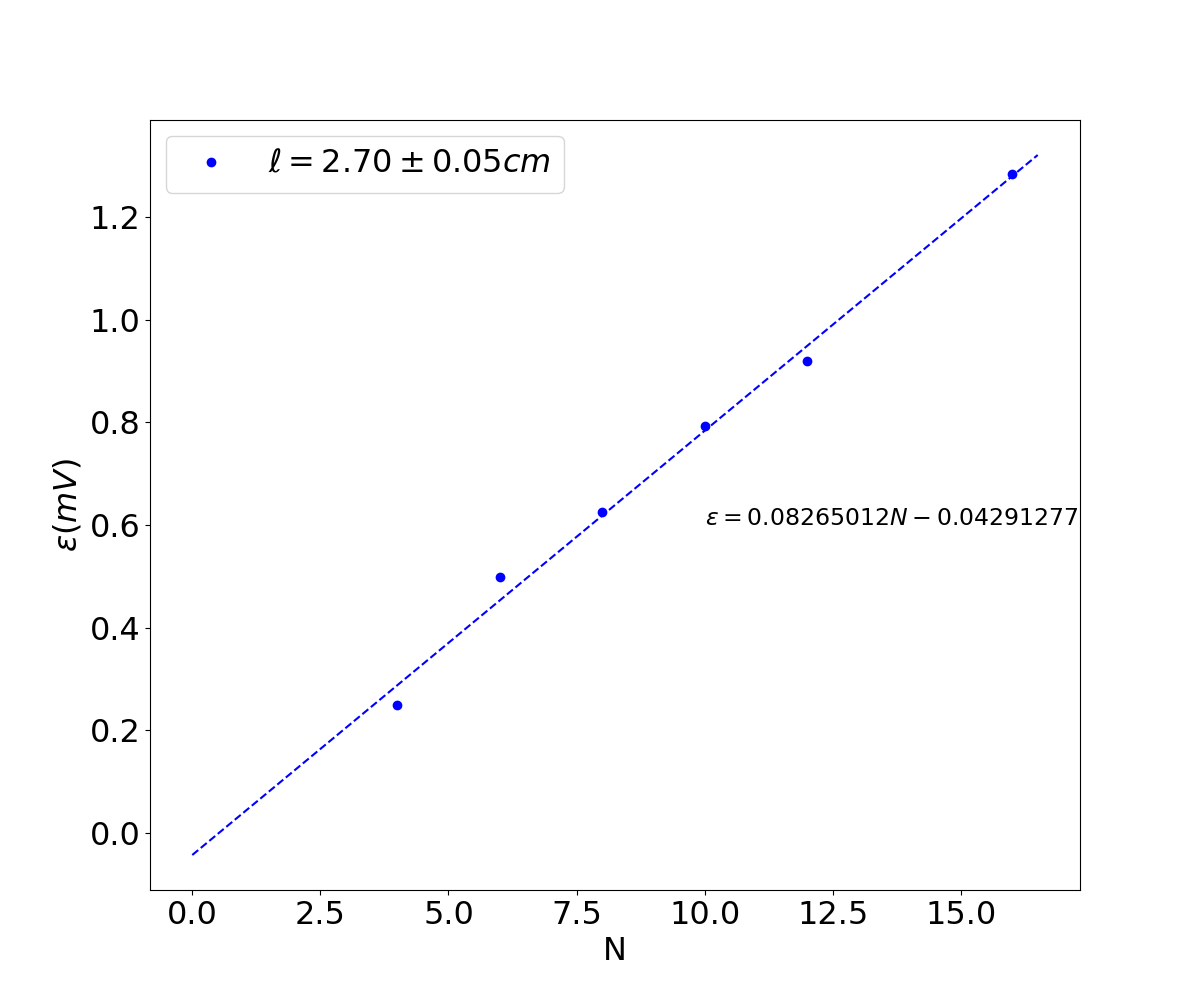
\includegraphics[scale=0.35]{bporimaneslconstante.png}
	\caption{Força Eletromotriz Induzida, $\epsilon$, em função do número de ímanes, $N$, na configuração com $\ell=2.70\pm0.05cm$.}
	\label{}
\end{figure}

\begin{figure}
	\center
	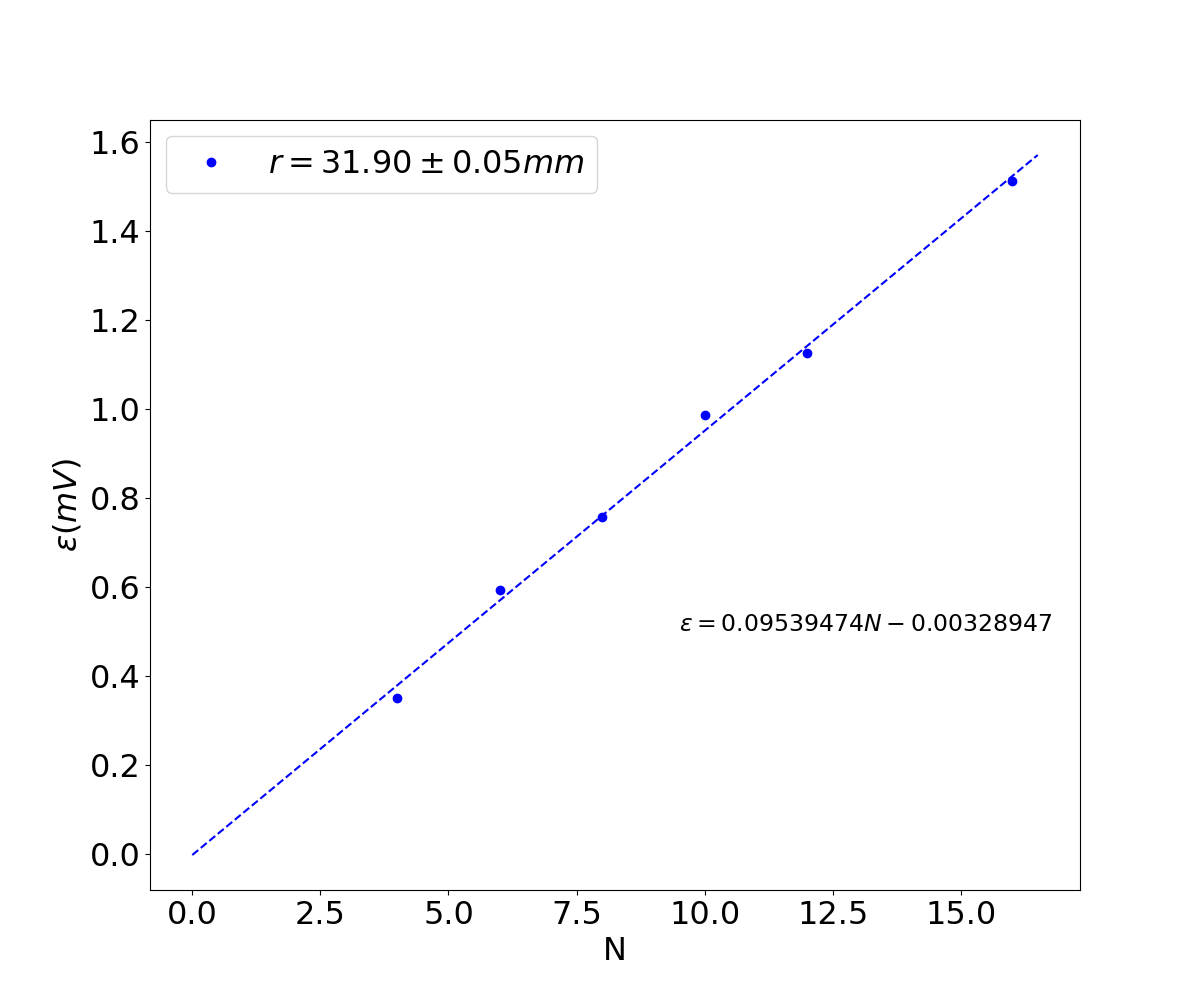
\includegraphics[scale=0.35]{bporimanesrconstante.png}
	\caption{Força Eletromotriz Induzida, $\epsilon$, em função do número de ímanes, $N$, na configuração com $r=31.90\pm0.05mm$.}
	\label{}
\end{figure}
Como podemos ver nos gráficos das figuras 4 e 5 a proporcionalidade direta também se verifica entre a força eletromotriz induzida e o número de ímanes no suporte.\\
Pelos campos magnéticos deduzidos em cada configuração calculou-se a média do campo gerado por um íman $B_{iman}=3.0664451783333333$ e respetivo desvio padrão $\sigma=0.3980653766660031$. Assim apresentamos o valor esperado do campo de um único íman $$B_{iman}=3.066 \pm 0.398 \;mT.$$
\chapter{Conclusão}
Após a análise feita no capítulo anterior confirma-se a proporcionalidade direta de primeira ordem entre a força eletromotriz induzida e a velocidade de arrastamento da espira, a área das espiras e o campo magnético.
Da mesma foi possível deduzir o campo magnético associado a cada íman: $B_{iman}=3.066 \pm 0.398 \;mT.$
%-------------------------------------%
%-------------BIBLIOGRAFIA------------%
\begin{thebibliography}{1}

  \bibitem{Abreu:1994} M.C. Abreu, L. Matias, L.F. Peralta {\it Física Experimental: Uma Introdução}. Editorial Presença, Lisboa: 1ª. ed., 1994. ISBN 972-23-1832-2.
  \bibitem{Serway:2014} R.A. Serway and J. W. Jewett, Jr. {\it Physics for Scientists and Engineers with Modern Physics}. Cengage, Boston: Tenth edition, 2014. ISBN 978-1-337-55329-2.
  \bibitem{Halliday:2014} Jearl Walker, David Halliday, Robert Resnick {\it Fundamentals of Physics}. Wiley, United States of America: 10th edition, 2014. ISBN 978-1-118-23072-5.


\end{thebibliography}
\end{document}
